\documentclass[../main.tex]{subfiles}
\graphicspath{{\subfix{../images/}}}
\begin{document}
\label{Ex:Equi}
Direct the focus of your concentration always on your center.

\noindent
\begin{tabular}{l p{9cm} }
 \raisebox{-\totalheight}{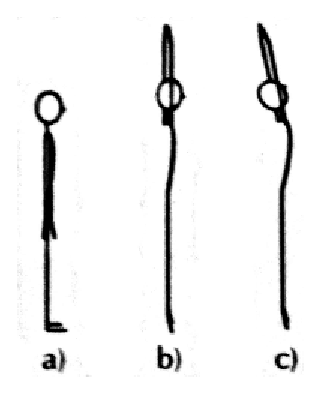
\includegraphics[width=3cm]{EqEx1}} & 
\begin{enumerate}[label=\alph*)]
\item Stand hip--wide and evenly distribute your weight on your feet. Consciously get in {contact with the floor} (gravity), ``root'' yourself.

Feel your {crown} and let yourself being ``pulled upwards'' (levitation).

Focus on your middle, the hara-centre (below your navel). Feel your {center}, breathe into it.

Imagine a {vertical axis}, from your feet to your crown.

\item Slowly and carefully {lift yourself} onto the tip of your toes.
                                      
\item Slowly direct your {gaze upward}.
\end{enumerate}
\\
\end{tabular}


\end{document}